\section{First iteration}
  After a few weeks of development the project grinded to a halt due to the framework established was incompatible with the ideas of how to improve the system. This led to the first refactor of the project. The code was working, but unable to be improved upon. I took what I learned from this first work and started planning the next iteration using the limitations of the first iteration as a spec for the next one. 

  The first iteration had some good features, but also lacked several important ones I found to be important after running into the first wall of the project. 
   
  \subsection{Features}
    The system was able to generate random melodies using stepwise motion, meaning moving by 2nds, and skips, meaning moving by 3rds. This made for somewhat singable melodies.

    \begin{figure}[h]
      \begin{center}
        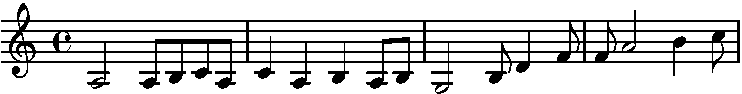
\includegraphics[width=0.95\textwidth]{examples/results/iteration1/melody.cropped.pdf}
      \end{center}
      \caption{Example melody of the first iteration melody generator.}\label{fig:iter1_melody}
    \end{figure}

  \subsection{Limitations}
    The system had no way to track which octave it was in which meant that longer melodies had a tendency to meader outside what would be considered as singable or even playable register. 

    There were no consideration of tension and release in the melody. Phrases never 

    Rests were not implemented in any way, pauses and rests are an important part of a melody and this needs to be addressed so that the melodies are not simply a continous stream of notes. 

  \subsection{Specifications for the second iteration}

    For the second iteration I wanted to focus on these things.

  \begin{itemize}
    \item No absolute notes until rendering(keep it at scale degrees, to reduce overhead)
    \item Octave tracking
    \item Restricted range
    \item Ending prases resolved(tonic, long note)
    \item Self similarity
  \end{itemize}

